\documentclass[journal]{IEEEtran}
\usepackage{subfigure}
\usepackage[pdftex]{graphicx}
\DeclareGraphicsExtensions{.pdf,.jpeg,.png}
\usepackage[center]{caption}
\begin{document}
%
% paper title
% can use linebreaks \\ within to get better formatting as desired
\title{Algoritmo de evasi\'on de obst\'aculos en tiempo real basado en visi\'on est\'ereo}

\author{Taih\'u Pire,~\IEEEmembership{FCEyN-UBA,}
        Sergio Gonz\'alez,~\IEEEmembership{FCEyN-UBA,}
        Emiliano Gonz\'alez,~\IEEEmembership{FCEyN-UBA,}
        Ra\'ul Benniti,~\IEEEmembership{FCEyN-UBA}% <-this % stops a space
        }

% The paper headers
%\markboth{Journal of \LaTeX\ Class Files,~Vol.~6, No.~1, January~2007}%
%{Shell \MakeLowercase{\textit{et al.}}: Bare Demo of IEEEtran.cls for Journals}

% make the title area
\maketitle


\begin{abstract}
En el presente trabajo se evaluar\'a un algoritmo de evasi\'on de obst\'aculos para navegaci\'on aut\'onoma de robots basado en mapas de profundidad. Aunque existen diversas tecnolog\'ias que permiten generar dichos mapas, los m\'etodos de visi\'on est\'ereo que generan mapas de disparidad han ganado relevancia en los \'ultimos a\~nos debido a la accesibilidad de los elementos de hardware necesarios, tanto como para obtener la informaci\'on sobre el entorno inmediato, como para procesarla. Se considerar\'an dos partes principales en el desarrollo propuesto: en primer lugar, se utilizar\'an las librer\'ias open source de procesamiento gr\'afico OpenCV y LIBELAS para, a partir de las im\'agenes provistas por una c\'amara \'estereo, generar mapas de disparidad de los que se pueda deducir informaci\'on relevante sobre la distancia de los objetos dentro de la ventana de visibilidad del robot; luego, se procesar\'an estos mapas para decidir si existe un obst\'aculo frente al robot y, de ser as\'i, divisar que acci\'on debe tomarse para evitarlo.
\end{abstract}

\begin{IEEEkeywords}
Mapa de disparidad, Visi\'on est\'ereo, Evasi\'on de obst\'aculos, Navegaci\'on aut\'onoma.
\end{IEEEkeywords}


\IEEEpeerreviewmaketitle


\section{Introducci\'on}
%comentar el uso de un sistema de navegacion, basado en camaras stereo. justificando (barato, accesible, costo computacional)

En la \'ultima d\'ecada se ha dado un gran impulso al \'area de rob\'otica abocada a la navegaci\'on aut\'onoma de veh\'iculos. Dado que el campo de aplicaci\'on es diverso, abarcando desde sistemas tan cr\'iticos como la exploraci\'on de lugares inaccesibles para veh\'iculos tripulados, hasta sistemas tan sencillos como la realizaci\'on de tareas dom\'esticas aut\'onomas, se han desarrollado tecnolog\'ias de distinta complejidad y costo operativo. En especial, se ha hecho principal incapi\'e en los sistemas basados en visi\'on, dada la variedad y el bajo costo que presentan las c\'amaras hoy en d\'ia.

En el presente informe se exhibe un algoritmo de evasi\'on de obst\'aculos basado \'unicamente en visi\'on est\'ereo para la navegaci\'on aut\'onoma de un robot. Visi\'on est\'ereo es una herramienta muy utilizada para la navegaci\'on aut\'onoma en los \'ultimos a\~nos debido al bajo costo de las c\'amaras y a la gran cantidad de informaci\'on que brindan. El software aqu\'i presentado para lograr la detecci\'on de obst\'aculos hace uso de una c\'amara est\'ereo permitiendo aproximar la distancia relativa en la que se encuentran los objetos con respecto a la c\'amara. Cabe destacar, que dicho algoritmo puede ser adaptado a cualquier dispositivo que cuente con una c\'amara del tipo mencionado. En lo que aqu\'i refiere, se utiliz\'o la c\'amara \emph{Minoru}, y como plataforma de prueba el robot \emph{exabot} \cite{DPSC09}.

%Otra de las ventajas de utilizar visi\'on est\'ereo para la navegaci\'on aut\'onoma, es la posibilidad de crear mapas 3D del entorno, si bien aqu\'i no se

El documento se encuentra estructurado de la siguiente manera: la secci\'on~\ref{sec:trabajajo_relacionado} introduce el estado del arte en sistemas de evasi\'on de obst\'aculos mediante el uso de visi\'on est\'ereo, la secci\'on~\ref{sec:hardware} detalla el hardware utilizado durante el desarrollo del algoritmo, la secci\'on~\ref{sec:pro_img} presenta las librer\'ias OpenCV y LIBELAS utilizadas para el procesamiento de im\'agenes y la generaci\'on de mapas de disparidad, la secci\'on~\ref{sec:heuristica} explica el algoritmo de evasi\'on de obst\'aculos propuesto, finalmente la secci\'on~\ref{sec:conclusiones} comenta algunas conclusiones y trabajo futuro.
\medskip

\hfill 20 de Julio de 2012

\section{Trabajo Relacionado}
\label{sec:trabajajo_relacionado}

Una de las \'areas de mayor inter\'es dentro del campo de la rob\'otica es la de navegaci\'on aut\'onoma. Con el pasar del tiempo se han propuesto y creado diversos sistemas de navegaci\'on que, adem\'as de las metodolog\'ias algor\'itmicas utilizadas (detecci\'on de caracter\'isticas, odometr\'ia, odometr\'ia visual, etc), se diferencian en las tecnolog\'ias elegidas para obtener la informaci\'on sobre el entorno. Algunas de las tecnolog\'ias m\'as utilizadas son:

\begin{itemize}
	\item \emph{C\'amaras de video}, que obtienen la informaci\'on en forma de im\'agenes. Los m\'etodos mas populares, utilizan una c\'amara (visi\'on monocular) o dos c\'amaras (visi\'on est\'ereo).
	
	\item Sensores de tipo \emph{sonar} o \emph{infrarojo}, para detectar objetos pr\'oximos.
	
	\item \emph{Radares} de microondas y radares \emph{l\'aser} (LIDAR).

	\item \emph{GPS}, en conjunto con un mapa del terreno por donde se desplazar\'a el robot.
\end{itemize}

Si bien los sistemas m\'as simples utilizan s\'olo alguna de \'estas tecnolog\'ias, distintos tipos de sensores pueden combinarse para obtener informaci\'on m\'as rica sobre el mundo. Todos \'estos pueden ser utilizados, adem\'as, en problemas de localizaci\'on y construcci\'on de mapas \cite{KNG10}.

Las c\'amaras est\'ereo representan un caso de inter\'es particular puesto que, dado que es posible calcular la profundidad relativa de los objetos en el \'area de visi\'on con un costo computacional relativamente bajo, pueden ser utilizadas de forma eficiente para la detecc\'ion de elementos en el espacio por donde se desplaza el robot. Partiendo de esta idea, en el trabajo actual se demuestra cómo es posible implementar un sistema de evasi\'on de obst\'aculos utilizando \'unicamente la informaci\'on provista por una c\'amara de \'estas caracter\'isticas.

En \cite{KNG10} se plantean tres t\'ecnicas para llevar a cabo la tarea de evasi\'on de obst\'aculos en base a la utilizaci\'on de mapas de profundidad o disparidad. El primer paso es com\'un a las tres: se propone dividir el mapa de disparidad en tres partes, una izquierda, una central y una derecha. La diferencia reside en como se procesa la informacion a partir de aqu\'i. En el primer m\'etodo propone calcular el promedio de disparidad en cada una de las zonas. Entonces, se dirigir\'e al robot en la direcci\'on correspondiente a la zona con el menor de los valores obtenidos, asumiendo que es aquella asociada a la menor cantidad de obst\'aculos. El segundo m\'etodo propuesto consiste en una evoluc\'ion del reci\'en comentado. En principio s\'olo se considera la parte central del mapa de disparidad. Se realiza un conteo sobre los p\'ixels que presentan una disparidad mayor a un cierto valor l\'imite, y se calcula el porcentaje que \'estos representan en relaci\'on al total de pixeles de esa zona particular. Si este porcentaje es alto (mayor a un valor previamente fijado), se deduce que frente a la c\'amara se encuentra un obst\'aculo. Es entonces que se decide realizar una acci\'on evasiva. Para poder elegir una direcci\'on hacia la cual girar, se analizan las zonas laterales y se procede hacia la que contenga el menor promedio de disparidad. El \'ultimo m\'etodo considera la condici\'on de que las tres zonas contengan un promedio de disparidad por encima de un umbral fijado. Si el robot se encuentra en este caso deber\'a reaccionar con una acci\'on de escape (por ejemplo, girar 180 grados para volver, o volver sobre el camino por donde se llego a la posici\'on actual). Una desventaja que puede observarse en los m\'etodos anteriores es que no se utiliza toda la informaci\'on disponible generada por la c\'amara est\'ereo, dado que solo se hace uso de un \'unico mapa de disparidad y esto puede llevar a problemas en la navegaci\'on. Para resolver dicho problema, en el procedimiento propuesto se utilizan ambos mapas de disparidad, rescatando la informaci\'on de cada uno para suplir las carencias mutuas (por ejemplo, si uno de los laterales contiene demasiado ruido en uno de los mapas, pero no en el otro).

En \cite{RH04} se plantea un m\'etodo para el procesamiento de las im\'agenes que utiliza una escala de grises para representar la distancia a la que se encuentra cada uno de los pixels. Adem\'as se sugiere no prestar atenci\'on a la informaci\'on que provenga del \'area del piso dado que, en general, no provee informaci\'on \'util si el terreno es plano y puede ser una fuente de ruido para el mapa de disparidad. Otra mejora al procesamiento de la informaci\'on proveniente de las c\'amaras consiste en realzar los bordes de la imagen. De esta manera, es posible reducir el ruido generado cuando se realizan movimientos bruscos hacia adelante o hacia los costados.

En \cite{H09} se sugiere el uso de solo una parte de la imagen, un \'area peque\~na en comparaci\'on al tama\~no total de la misma. \'Esto es lo que se conoce como regi\'on de inter\'es. Aunque no se disminuye la complejidad del proceso, sí se logra reducir el tiempo requerido para poder obtener el resultado. Un problema que podr\'ia presentar este proceder es que, si el \'area de inter\'es es demasiado peque\~na, se omita informaci\'on relevante sobre la escena a procesar. El m\'etodo aqu\'i propuesto tambi\'en utiliza una reducci\'on de las areas a procesar, con el fin de no inclu\'ir la informaci\'on superflua proveniente del terreno propiamente dicho.

\section{Hardware Utilizado}
% Descripcion del robot, descripcion de la minoru, explicacion (breve) de la calibracion (uso de toolbox calib)
\label{sec:hardware}


Durante el desarrollo de este trabajo se utiliz\'o el robot {\bf Exabot}, dise\~nado y fabricado en la facultad FCEyN-UBA, Argentina. Se trata de un veh\'iculo m\'ovil con cuatro ruedas, unidas por dos orugas, y dos motores, lo que permite movimientos con dos grados de libertad en el plano. Se configur\'o con una c\'amara est\'ereo y montaje para computadoras port\'atiles. La interfaz de comunicaci\'on con el mismo es v\'ia red, que se utiliza \'unicamente para enviar comandos.

\begin{figure}[ht]
	\begin{center}
		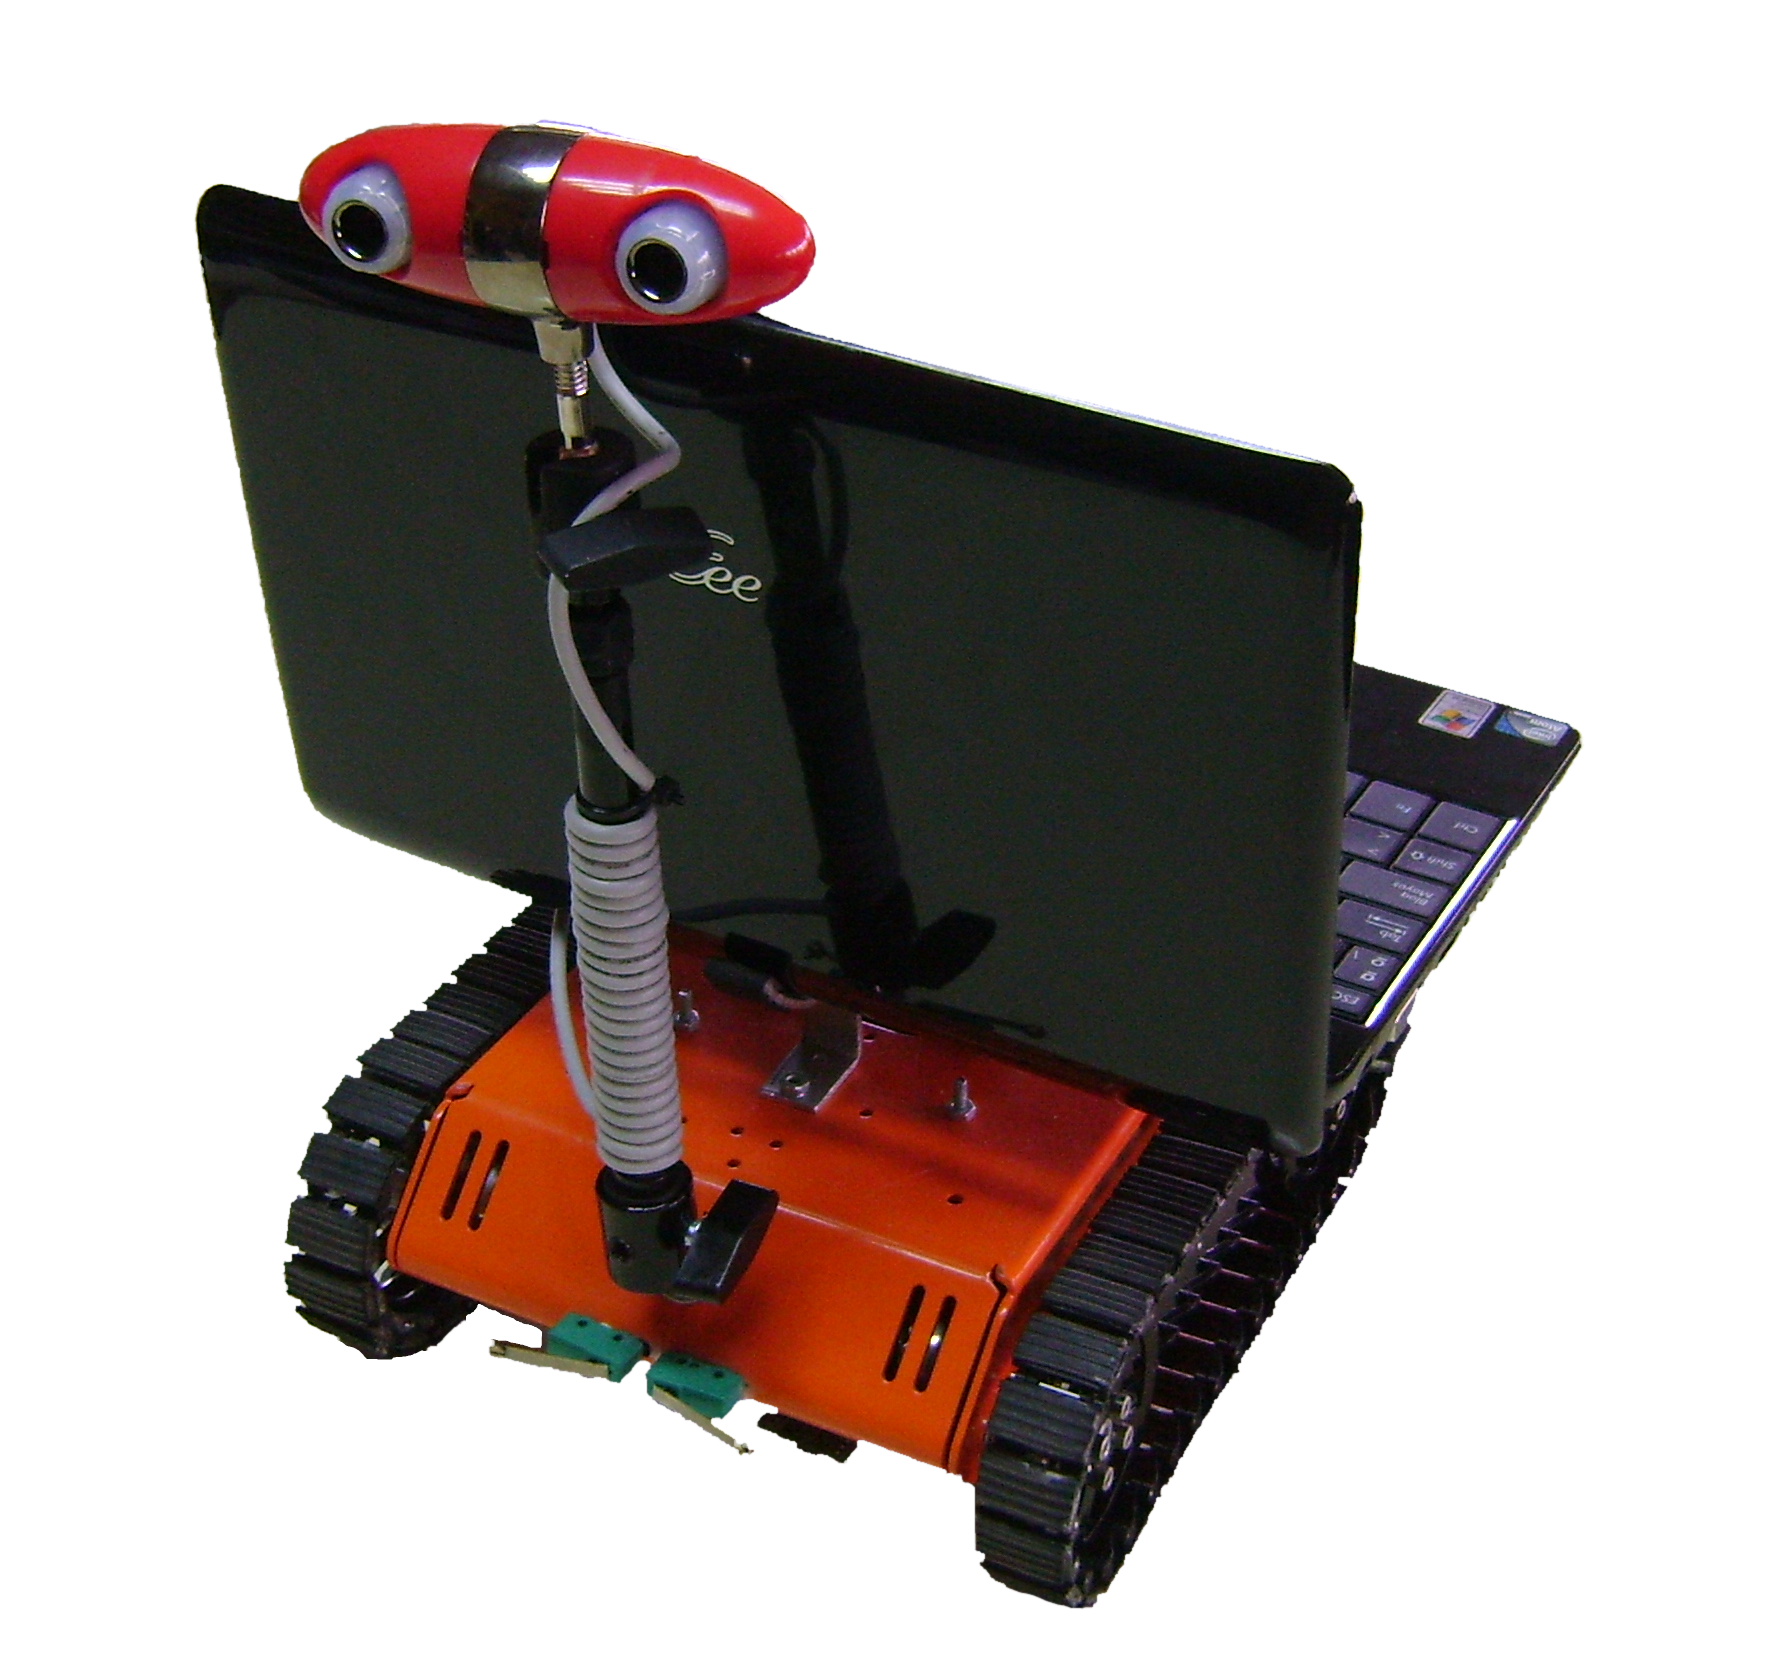
\includegraphics[width=6cm]{./images/exabot_04.png}
		\includegraphics[width=6cm]{./images/exabot_03.png}
		\caption{Configuraci\'on de Exabot utilizada}
	\end{center}
\end{figure}

El equipo de visi\'on est\'ereo montado en este trabajo es una c\'amara est\'ereo {\bf Minoru}. La misma se conecta v\'ia USB a la computadora port\'atil. Sus caracter\'isticas son las siguientes: 60 mm de base est\'ereo, USB 2.0, resoluciones desde 320x240 a 1280x480, 15~30fps, 1.5 W en modo operativo y 2 mW en modo suspendido. La resoluci\'on utilizada en este trabajo para las im\'agenes es de 640x480, capturadas a 15fps. Cabe aclarar que si bien la cantidad de im\'agenes disponibles por segundo es la mencionada anteriormente, las que realmente se procesan en general son menos, debido a la complejidad del algoritmo y el poder de c\'omputo del hardware.

En el contexto de algoritmos de Visi\'on, es mandatario calibrar las c\'amaras para poder identificar sus par\'ametros intr\'insecos (relativos a la c\'amara: distancia focal, punto principal, distorsi\'on radial) y extr\'insecos (de la c\'amara con respecto al mundo: rotaci\'on y traslaci\'on). Estos par\'ametros son luego utilizados para realizar las correctas transformaciones proyectivas a la imagen, que logran extraer informaci\'on de cada p\'ixel.

En este trabajo, utilizamos la matriz de calibraci\'on de cada c\'amara para rectificar las im\'agenes y calcular su mapa de disparidad correspondiente, como veremos en la secci\'on~\ref{sec:pro_img}.

La calibraci\'on de las c\'amaras se realiz\'o utilizando un paquete de MATLAB llamado {\bf Toolbox Calib} \cite{B00}. El producto de esta calibraci\'on est\'ereo es un archivo con los valores de los par\'ametros para ambas c\'amaras. Con este archivo se procede a generar otro con formato XML de una estructura en particular, que permite leerlo con la librer\'ia OpenCV.

\section{Procesamiento de las Ima\'genes}
\label{sec:pro_img}
%explicar la rectificacion vertical y alineacion horizontal usando libelas y opencv y la generacion de mapas de disparidad

Para realizar un algoritmo de evasi\'on de obst\'aculos, en este trabajo se utilizan mapas de disparidad, que contienen informaci\'on de profundidad para cada uno de los pixeles con respecto a la c\'amara. Esto es posible gracias a la visi\'on est\'ereo. Una de las pre-condiciones consiste en tener ambas im\'agenes de forma tal que, los pixels que se correspondan entre una im\'agen y otra se encuentren a la misma altura. Se llama disparidad a la distancia de un pixel en una imagen con su correspondiente en la otra. Aquellos pertenecientes a un objeto cercano, tendr\'an mayor disparidad que otros pertenecientes a un objeto lejano. Los puntos en com\'un en cada imagen se buscan por medio de un algoritmo de correspondencia.

La precondici\'on se debe cumplir antes de generar el mapa, por esta razo\'n debe realizarce una rectificaci\'on de ambas im\'agenes, una alineaci\'on vertical (de ambas) y horizontal (de la im\'agen derecha sobre la izquierda), de forma que una l\'inea se encuentre a la misma altura en una imagen y en otra. Estos par\'ametros son obtenidos con la ayuda de la librer\'ia $OpenCV$ \cite{opencv}.

En general, un \'ultimo paso es necesario. Una alineaci\'on horizontal de una imagen sobre otra para definir que se considera como disparidad cero, es decir la distancia mas lejana que se quiere representar. Dicho valor puede variar dependiendo el ambiente en el cual se trabaje, por ejemplo, si el ambiente es de interior, es probable, que la disparidad cero se encuentre a una distancia mas cercana que si el ambiente es exterior, y esto resulta en una alineaci\'on diferente para cada caso.

%mapas de disparidad

\begin{figure}[ht]
	\begin{center}
		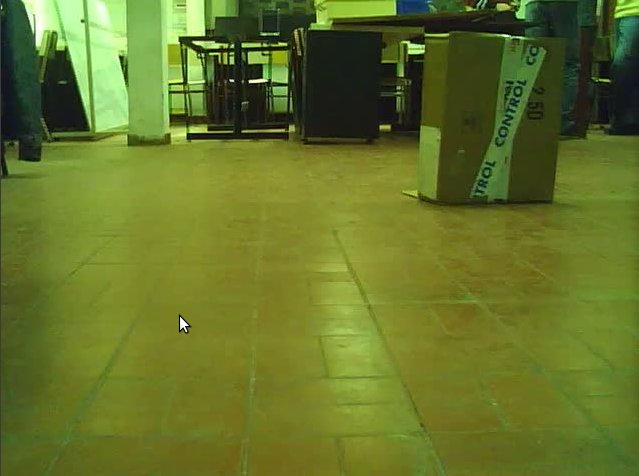
\includegraphics[width=6cm]{./images/original.jpg}
		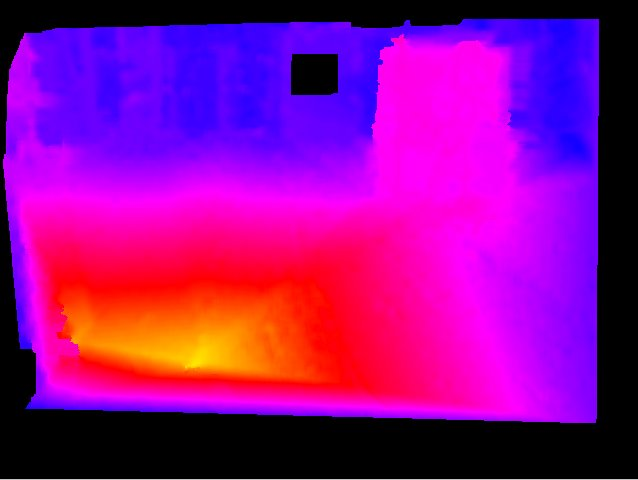
\includegraphics[width=6cm]{./images/disparidad.jpg}
		\caption{Captura de la c\'amara izquierda de la c\'amara Minoru (imagen superior) y su correspondiente mapa de disparidad (imagen inferiror).}
	\end{center}
\end{figure}

\section{Heur\'istica de Evasi\'on de Obst\'aculos}
%Explicacion de como se usa el mapa de disparidad (partiendo en 3 zonas etc.)(decir que solo se utiliza el mapa de un solo lado, izquierdo)
\label{sec:heuristica}

La heur\'istica de evasi\'on de obst\'aculos que se implementa est\'a basada en el M\'etodo de Estimaci\'on por Umbral (\emph{Threshold Estimation Method}) analizado en \cite{KNG10}. \'Este m\'etodo utiliza mapas de disparidad para aproximar la distancia a la que se encuentran los objeto capturados por la c\'amara est\'ereo. En lo que sigue, se presentan las variaciones implementadas sobre el algoritmo.

En primer lugar, se divide el mapa de disparidad en tres ventanas verticales con base variable, tal como se muestra en la figura~\ref{fig:piernas_cerca}. El ancho de la ventana central es mayor que el de las ventanas laterales, dado que la c\'amara cuenta con un \'angulo de visi\'on reducido, logrando as\'i que el algoritmo obtenga mayor informaci\'on sobre los objetos que se encuentran delante y representan obst\'aculos potenciales. Adem\'as se modificaron independientemente los tama\~nos de las ventanas de los lados, con el fin de reducir el ruido generado por la falta de informaci\'on en los bordes de las im\'agenes. Por otro lado, se defini\'o un l\'imite para determinar la regi\'on de interes sobre la cual se procesan los datos \cite{H09}, prescindiendo de la informaci\'on ``ruidosa'' producida por el suelo (se considera que el robot se desplaza sobre un terreno plano).

\begin{figure}[ht]
	\begin{center}
		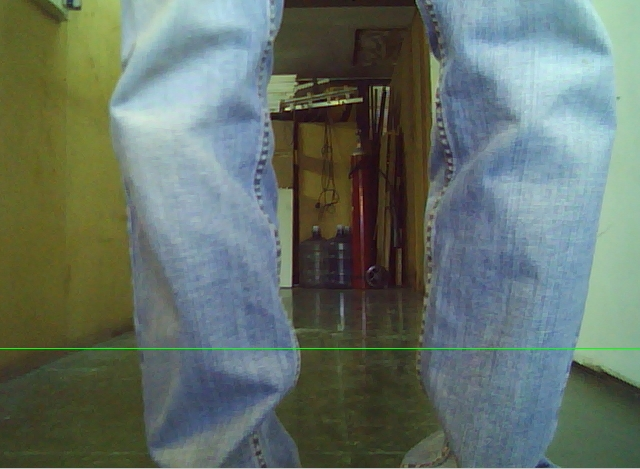
\includegraphics[width=6cm]{./images/piernas_cerca.jpg}
	\end{center}
	\caption{Ventanas de una imagen. La linea horizontal representa la regi\'on de interes.}
	\label{fig:piernas_cerca}
\end{figure}

El segundo paso consiste en estimar los porcentajes de p\'ixeles del mapa de disparidad que representen objetos cercanos, los cuales se obtienen para cada una de las ventanas por separado. Para \'esto, sobre cada \'area se contabilizan los p\'ixeles que posean una disparidad mayor a un cierto umbral de tolerancia; mientras menor sea el umbral, mayor ser\'a la cantidad de p\'ixeles considerados cercanos. Al observar que el algortimo de procesamiento de las im\'agenes genera un alto grado de ruido para los objetos pr\'oximos a la c\'amara, se decidi\'o incluir tambi\'en aquellos p\'ixeles que no cuenten con informaci\'on de disparidad. Para evitar que \'estos tomen predominancia sobre los p\'ixeles de alta disparidad, se los incorpora ponderandolos al $30\%$ del valor de un p\'ixel con disparidad alta. Cabe destacar que por motivos de eficiencia las zonas de los lados no son procesadas hasta el momento en que realmentes sea necesario disponer de su informaci\'on. En la figura~\ref{fig:piernas} se puede observar dicho comportamiento.


\begin{figure}[ht]
\centering
\subfigure[Una persona a $1.5$ metros de distancia a la c\'amara, junto con su correspondiente mapa de disparidad.]{
    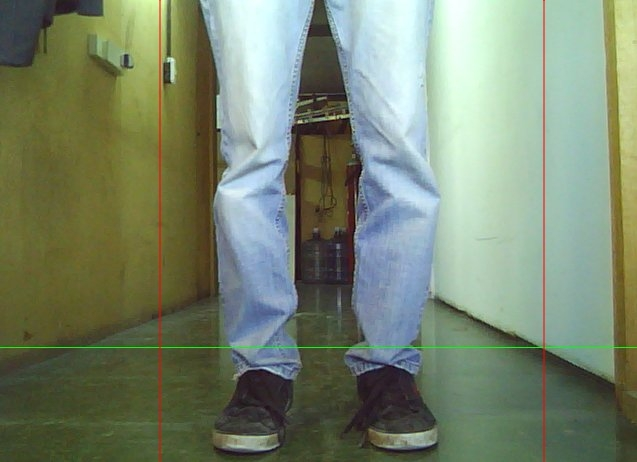
\includegraphics[width=4cm]{./images/piernas_lejos.jpg}
    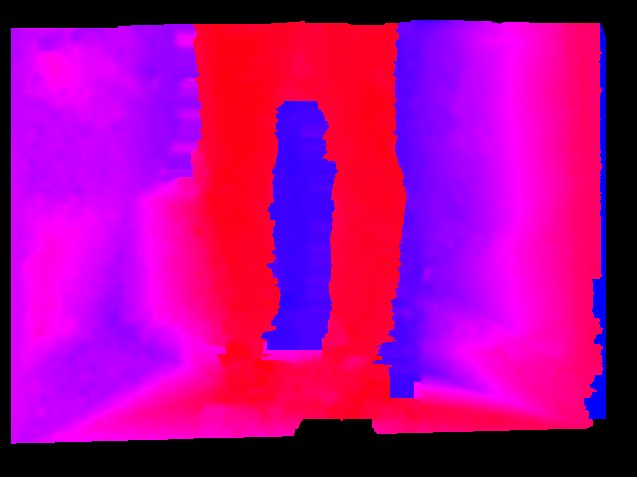
\includegraphics[width=4cm]{./images/piernas_disparidad_lejos.jpg}
    \label{fig:subfig1}
}
\subfigure[Cuando la persona se encuentra cercana a la c\'amara (a $50$ cent\'imetros aproximadamente), se puede observar, que en la ventana central de la imagen predom\'inan p\'ixeles con disparidad alta, como se puede ver en el mapa de disparidad (p\'ixeles verdes).]{
    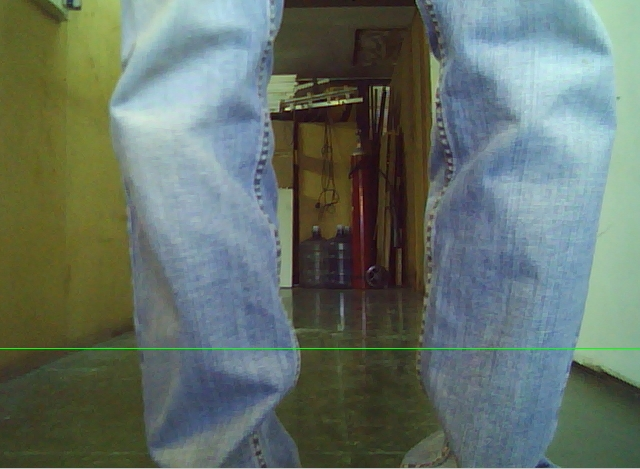
\includegraphics[width=4cm]{./images/piernas_cerca.jpg}
    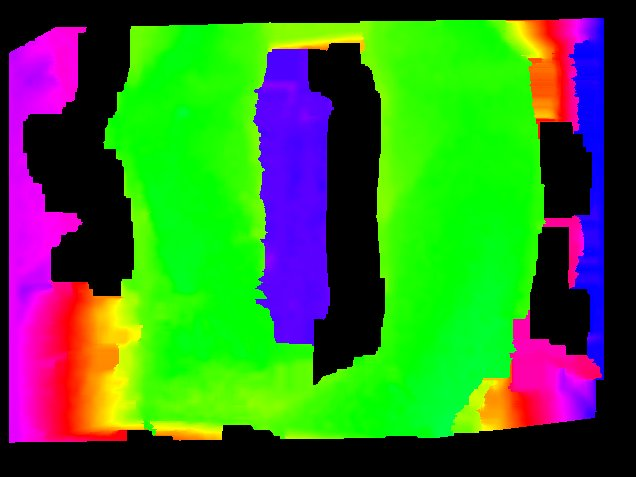
\includegraphics[width=4cm]{./images/piernas_disparidad_cerca.jpg}
    \label{fig:subfig2}
}

\caption{Im\'agenes donde se muestran las ventanas y el \'area de interes procedas en cada momento.}
\label{fig:piernas}
\end{figure}

Una vez obtenidos los porcentajes, se procede a la toma de la decisi\'on propiamente dicha. En principio se analiza \'unicamente la zona central. Si el porcentaje de p\'ixeles con disparidad alta es menor a un valor predeterminado (por ejemplo, $30\%$), se considera que el camino se encuentra sin obst\'aculos cercanos y el robot puede continuar su desplazamiento en linea recta. En cambio, si el umbral es superado, se procede a comparar los porcentajes de p\'ixeles de alta disparidad de las ventanas laterales (cada uno respecto a la cantidad de p\'ixeles total de la ventana correspondiente), a diferencia de \cite{KNG10}. La ventana con menor valor asociado representa la direcci\'on con menos obst\'aculos, y por lo tanto se procede a girar el robot (sobre su eje) en dicho sentido. Cabe aclarar, que la velocidad angular del robot es mayor a la velocidad de traslaci\'on. \'Esta fue seleccionada con la intenci\'on de mitigar la informaci\'on borrosa (blur) generada por el movimiento de rotaci\'on, que conlleva a la obtenci\'on de mapas de disparidad con una gran cantidad de ruido.


\section{Conclusiones}
%comentar que se pueden usar los dos mapas (de la parte derecha e izquierdas, etc)
\label{sec:conclusiones}
Se desarrollo un algoritmo para la evasi\'on de obst\'aculos basado en mapas de disparidad. Para el procesamiento de los mapas de profundida, se utilizaron las librer\'ias OpenCV (Open Source Computer Vision) que cuenta con funciones para visi\'on en computadora en tiempo real y LIBELAS (Library for Efficient LArge-scale Stereo Matching) espec\'ifica para la manipulaci\'on de imagenes est\'ereo de gran resoluci\'on. Por otro lado, se realizaron experimentos que verificaron el correcto comportamiento del m\'etodo implementado para la evasi\'on de obst\'aculos en tiempo real. Como trabajo futuro se podr\'ia integrar la informaci\'on provista por los mapas de disparidad resultantes de las imagenes izquierda y derecha logrando as\'i una mejor aproximaci\'on de profundidad. Adem\'as queda abierta la posibilidad de incorporar un m\'etodo de localizaci\'on y construcci\'on simult\'anea de Mapas, SLAM (por sus siglas en ingl\'es de Simultaneous localization and mapping) junto con un mecanismo de planeamiento de navegaci\'on.





\nocite{KNG10}
\nocite{G10}
\nocite{opencv}
\nocite{B00}
\nocite{H04}
\nocite{DPSC09}
\nocite{RH04}
\nocite{H09}

\bibliographystyle{unsrt}
\bibliography{biblio}

%\begin{thebibliography}{1}
%
%\bibitem{IEEEhowto:kopka}
%H.~Kopka and P.~W. Daly, \emph{A Guide to \LaTeX}, 3rd~ed.\hskip 1em plus
%  0.5em minus 0.4em\relax Harlow, England: Addison-Wesley, 1999.
%
%\end{thebibliography}

% that's all folks
\end{document}